\documentclass{article}
\pagenumbering{arabic}
\usepackage{graphicx,amsmath,amssymb,bm,tikz,stmaryrd,pict2e,picture}
\usetikzlibrary{calc,patterns,decorations.pathmorphing,decorations.markings}
\usepackage{xfrac}
\usepackage[utf8]{inputenc}
\usepackage{hyperref}
% Format fref 
\usepackage[plain,english]{fancyref}
\usepackage[margin=1in]{geometry} 
\fancyrefaddcaptions{english}{\renewcommand*{\frefeqname}{Eq.}}
% Figure Packages
\usepackage[outercaption]{sidecap}
\usepackage[export]{adjustbox}
\usepackage{graphicx}
\usepackage{caption}
\usepackage{wrapfig}
\usepackage{float}
\usepackage{algorithm, algorithmic, amsfonts,amsmath,amssymb,amsthm, color,comment,enumitem, environ, fancyhdr,   graphicx, mathtools, wasysym}
\pagestyle{fancy}
\setlength{\headheight}{22.5pt}
\newenvironment{problem}[2][Problem]{\begin{trivlist}
\item[\hskip \labelsep {\bfseries #1}\hskip \labelsep {\bfseries #2.}]}{\end{trivlist}}
\newenvironment{sol}
    {\emph{Solution:}
    }
    {
    \qed
    }
\specialcomment{com}{ \color{blue} \textbf{Comment:} }{\color{black}} %for instructor comments while grading
\NewEnviron{probscore}{\marginpar{ \color{blue} \tiny Problem Score: \BODY \color{black} }}
%%%%%%%%%%%%%%%%%%%%%%%%%%%%%%%%%%%%%%%%%%%%%%%%%%%%%%%%%%%%%%%%%%%%%%%%%%%%%%%%%





%%%%%%%%%%%%%%%%%%%%%%%%%%%%%%%%%%%%%%%%%%%%%
%Fill in the appropriate information below
\lhead{Daniel Agramonte}  %replace with your name
\rhead{EE 363 \\ Homework 1} %replace XYZ with the homework course number, semester (e.g. ``Spring 2019"), and assignment number.
%%%%%%%%%%%%%%%%%%%%%%%%%%%%%%%%%%%%%%%%%%%%%



% Table stuff
\usepackage{multirow}
%\usepackage{floatrow}
%	\floatsetup[table]{capposition=top}%puts table caption above
% Change \subsection title characteristics
    \usepackage[parfill]{parskip}   % forces parskip to not affect headings
    \usepackage{enumitem}           % used for editing itemize environment
    \usepackage{titlesec}
        \titleformat*{\section}{\Large\bfseries\titlerule\vspace{0.5em}}
% Quote blocks
    \usepackage{csquotes} % use environment 'displayquote'
% Misc document settings
    \title{\Huge EE 363 Homework 1} \author{Daniel Agramonte} \date{2.03.21}
    \setlength{\parindent}{0pt}
    \setlength{\parskip}{1em}
    \setlist{nosep, itemsep=0pt, parsep=0pt}
% Misc vocab commands
    \newcommand{\msalg}{{\fontfamily{cmtt}\selectfont ms83}}
    \newcommand{\lsq}{\emph{lsqnonlin}}
    \newcommand{\msalge}{{\fontfamily{cmtt}\selectfont MCHE\_6500\_NIST\_POLY}}
%
% MATLAB packages
%
\usepackage[framed,numbered]{matlab-prettifier}
\usepackage{textcomp}
\usepackage{listings}
%
% Matrix Spacing
%
\makeatletter
\renewcommand*\env@matrix[1][\arraystretch]{%
  \edef\arraystretch{#1}%
  \hskip -\arraycolsep
  \let\@ifnextchar\new@ifnextchar
  \array{*\c@MaxMatrixCols c}}
\makeatother
%

\newcommand{\varslash}{%
  \mathbin{\mathpalette\pictslash{{0}{1}}}%
}
\newcommand{\varbslash}{%
  \mathbin{\mathpalette\pictslash{{1}{-1}}}%
}

\makeatletter
\newcommand{\pictslash}[2]{%
  \vcenter{\hbox{%
    \sbox0{$\m@th#1\varobslash$}\dimen0=.55\wd0
    \pictslash@aux#2%
  }}%
}
\newcommand{\pictslash@aux}[2]{%
    \begin{picture}(\dimen0,\dimen0)
    \roundcap
    \put(0,#1\dimen0){\line(1,#2){\dimen0}}
    \end{picture}%
}
\makeatother
\begin{document}
\maketitle

\begin{enumerate}
    \item \textit{LQR for a triple accumulator}. We consider the system $x_{t+1}=Ax_{t}+Bu_{t}$, $y_{t}=Cx_{t}$, with
    \begin{flalign*}
        A = 
        \begin{bmatrix}
            1 & 0 & 0 \\
            1 & 1 & 0 \\
            0 & 1 & 1
        \end{bmatrix},\qquad
        B = 
        \begin{bmatrix}
            1 \\
            0 \\
            0
        \end{bmatrix},\qquad
        C = 
        \begin{bmatrix}
            0 & 0 & 1
        \end{bmatrix}.
    \end{flalign*}
    This system has a transfer function $H(z)=(z-1)^{-1}$, and is called a triple accumulator, since it consists of a cascade of three accumulators. (An accumulator is the discrete-time analog of an integrator: its output is the running sum of its input.) We'll use the LQR cost function
    \begin{flalign*}
        J = \displaystyle{\sum_{t=0}^{N-1}u_{t}^{2}}+\displaystyle{\sum_{t=0}^{N}y_{t}^{2}},
    \end{flalign*}
    with $N=50$.
    \\
    \begin{enumerate}
        \item Find $P_t$ (numerically), and verify that the Riccati recursion converges to a steady-state feedback gain $K_{t}$, and plot its components $(K_{t})_{11}$, $(K_{t})_{12}$, and $(K_{t})_{13}$, versus $t$.
        \\
        \\
        \begin{sol}
            we first note that $\rho=1$.
            \\
            \\
            Verified:
            $P_{t}$ converges to 
            \begin{flalign*}
                \begin{bmatrix}
                    6.764 & 7.689 & 2.786 \\
                    7.689 & 11.527 & 5.187 \\
                    2.786 & 11.527 & 5.187
                \end{bmatrix}.
            \end{flalign*}
            We may take error in the following fashion to show convergence:
            \begin{flalign*}
                \varepsilon_{P,t} &= \max\left(\left(\left(P_{t+1}-P_{t}\right)\varobslash P_{t}\right)^{|\cdot|}\right),&&
            \end{flalign*}
            where $X^{|\cdot|}$ refers to the element-wise absolute value of a matrix $X$.
            \\
            \\
            Taking $\varepsilon_{P,t}$ in this fashion let's us see that our error falls below 0.1\% after 9 iterations of our algorithm, i.e. when $t=40$.
            \\
            \\
            Similarly, we have the convergence of $K_{t}$ to
            \begin{flalign*}
                \begin{bmatrix}
                    -1.861 & -1.349 & -0.359
                \end{bmatrix}.
            \end{flalign*}
            Again, taking our error to be
            \begin{flalign*}
                \varepsilon_{K,t} &= \max\left(\left(\left(K_{t+1}-K_{t}\right)\varobslash K_{t}\right)^{|\cdot|}\right),&&
            \end{flalign*}
            we find that our error falls below 0.1\% after 9 iterations.
                \begin{figure}[H]
                    \vspace{-10pt}
                    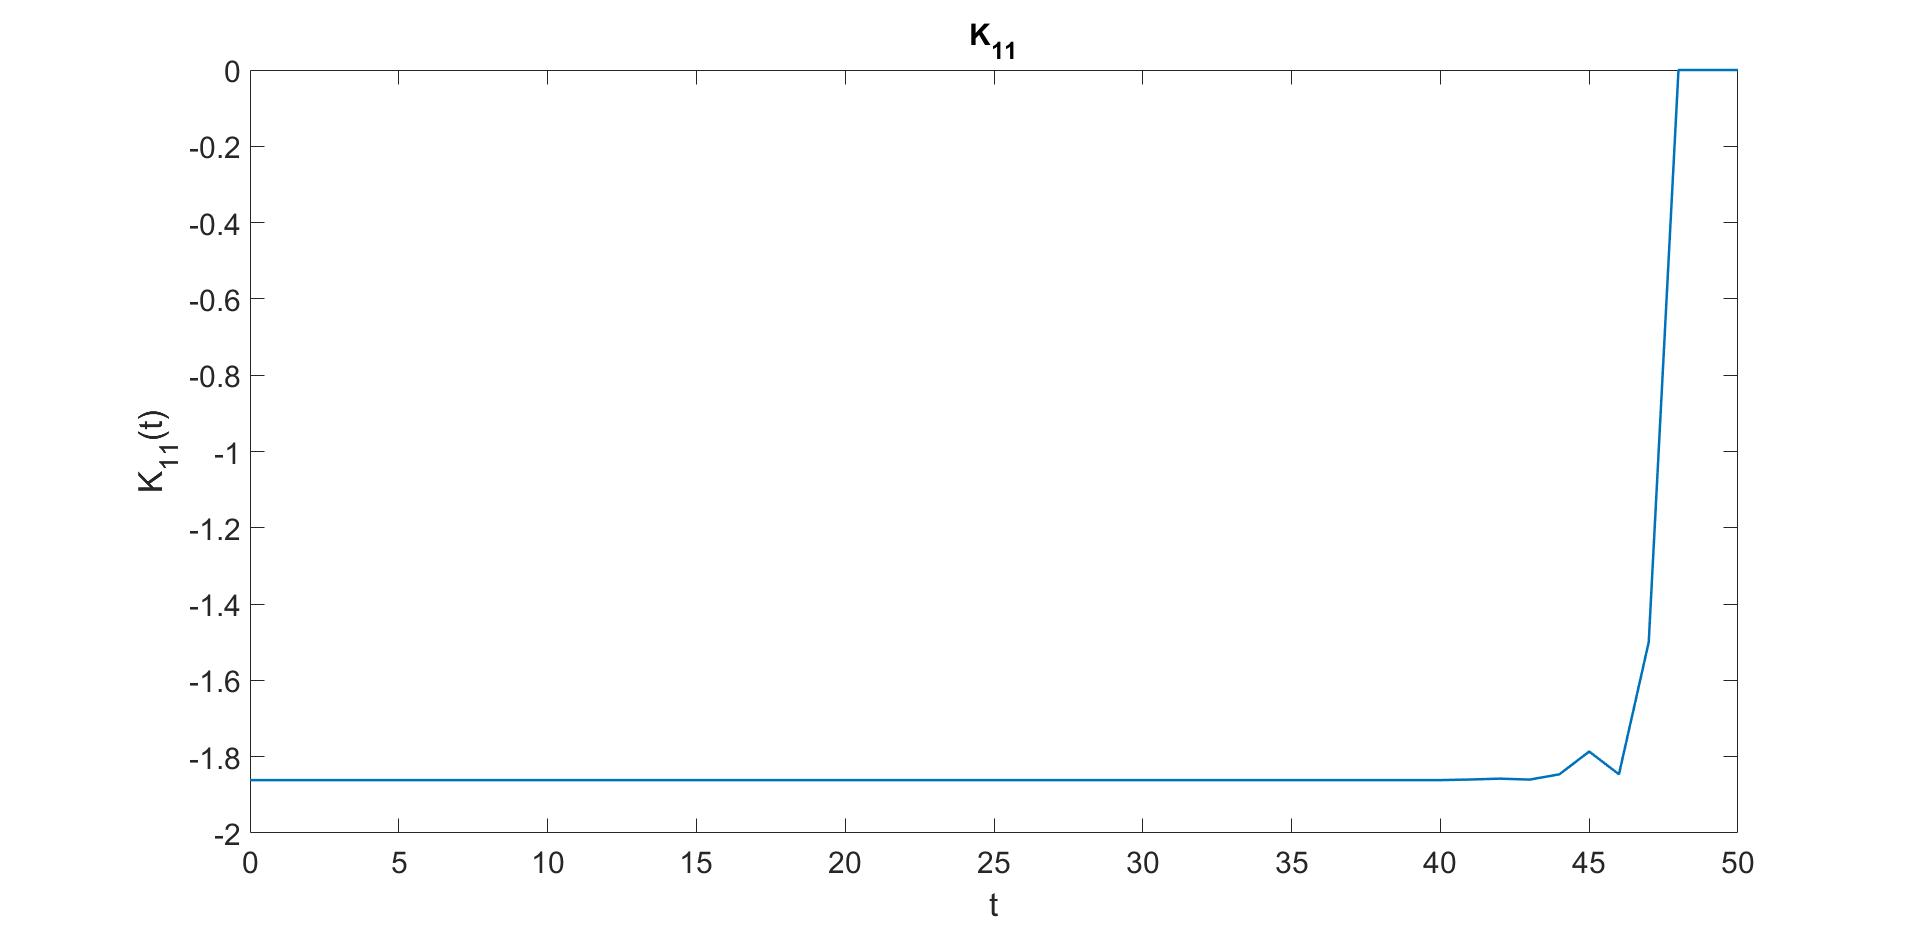
\includegraphics[width=\textwidth,left]{EE 363/HW1/Figures/Figure 1.jpg}
                    \label{fig:Fig_1}
                \end{figure}
                \begin{figure}[H]
                    \vspace{-10pt}
                    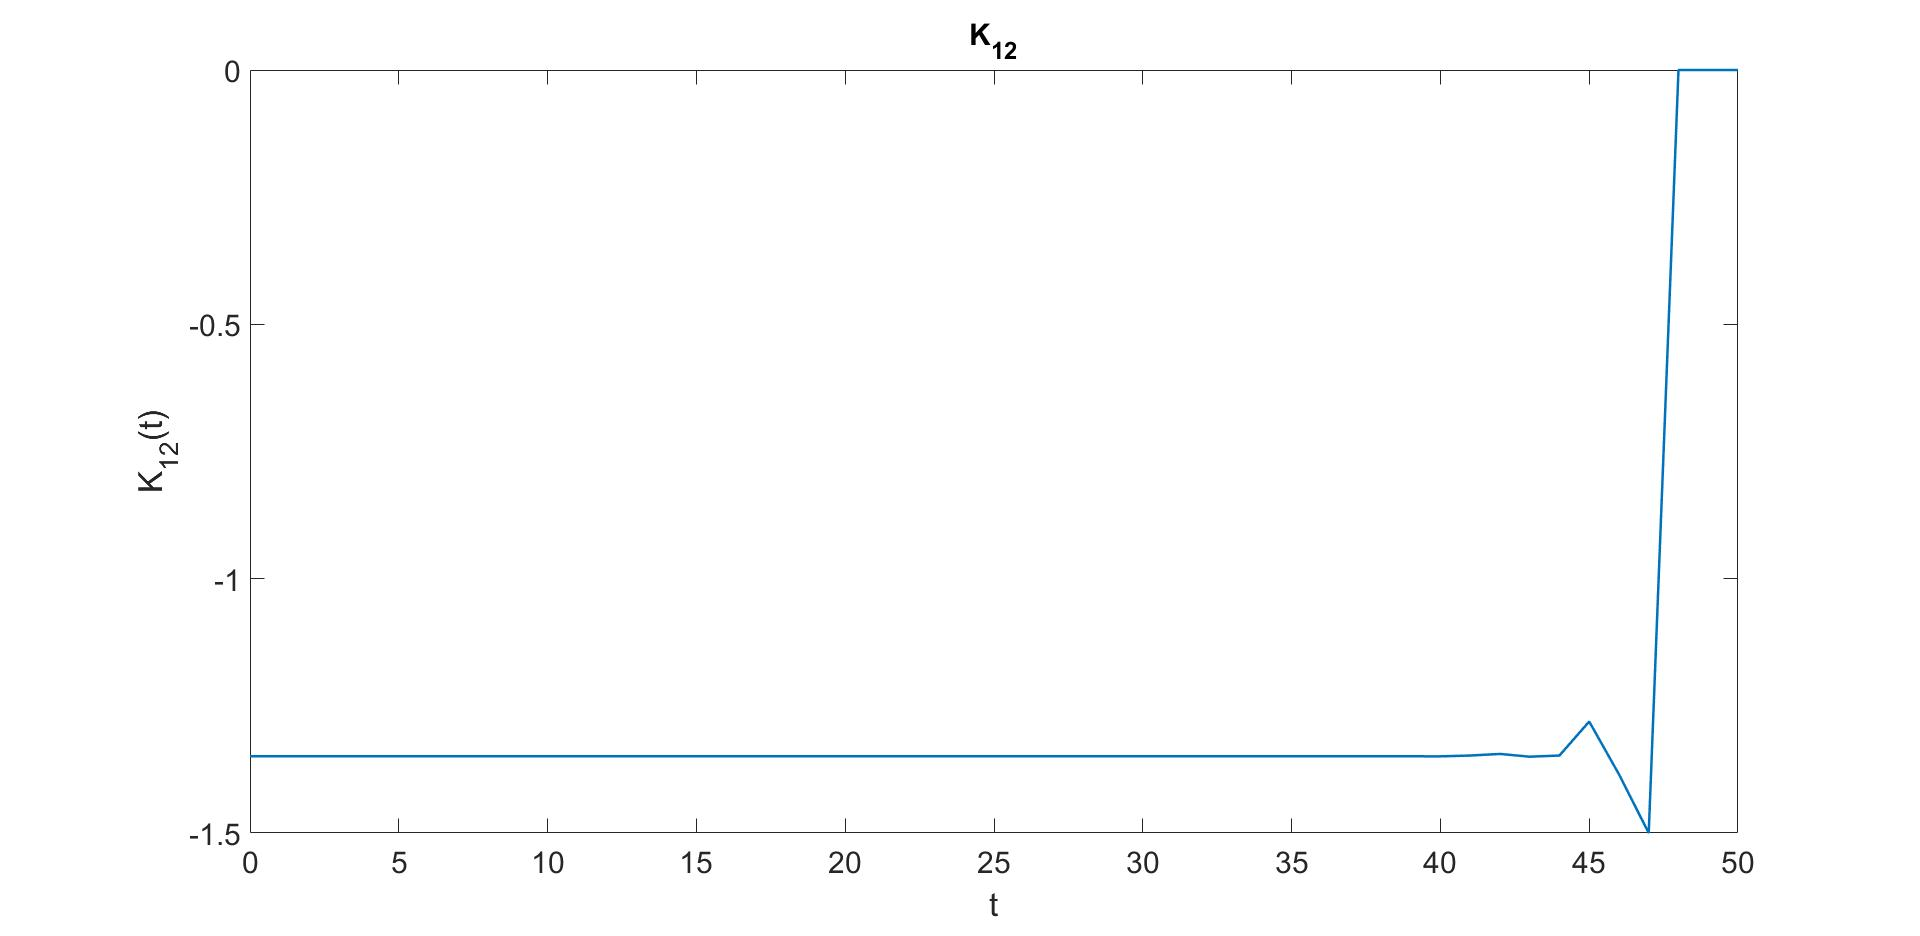
\includegraphics[width=\textwidth,left]{EE 363/HW1/Figures/Figure 2.jpg}
                    \label{fig:Fig_2}
                \end{figure}
                \begin{figure}[H]
                    \vspace{-10pt}
                    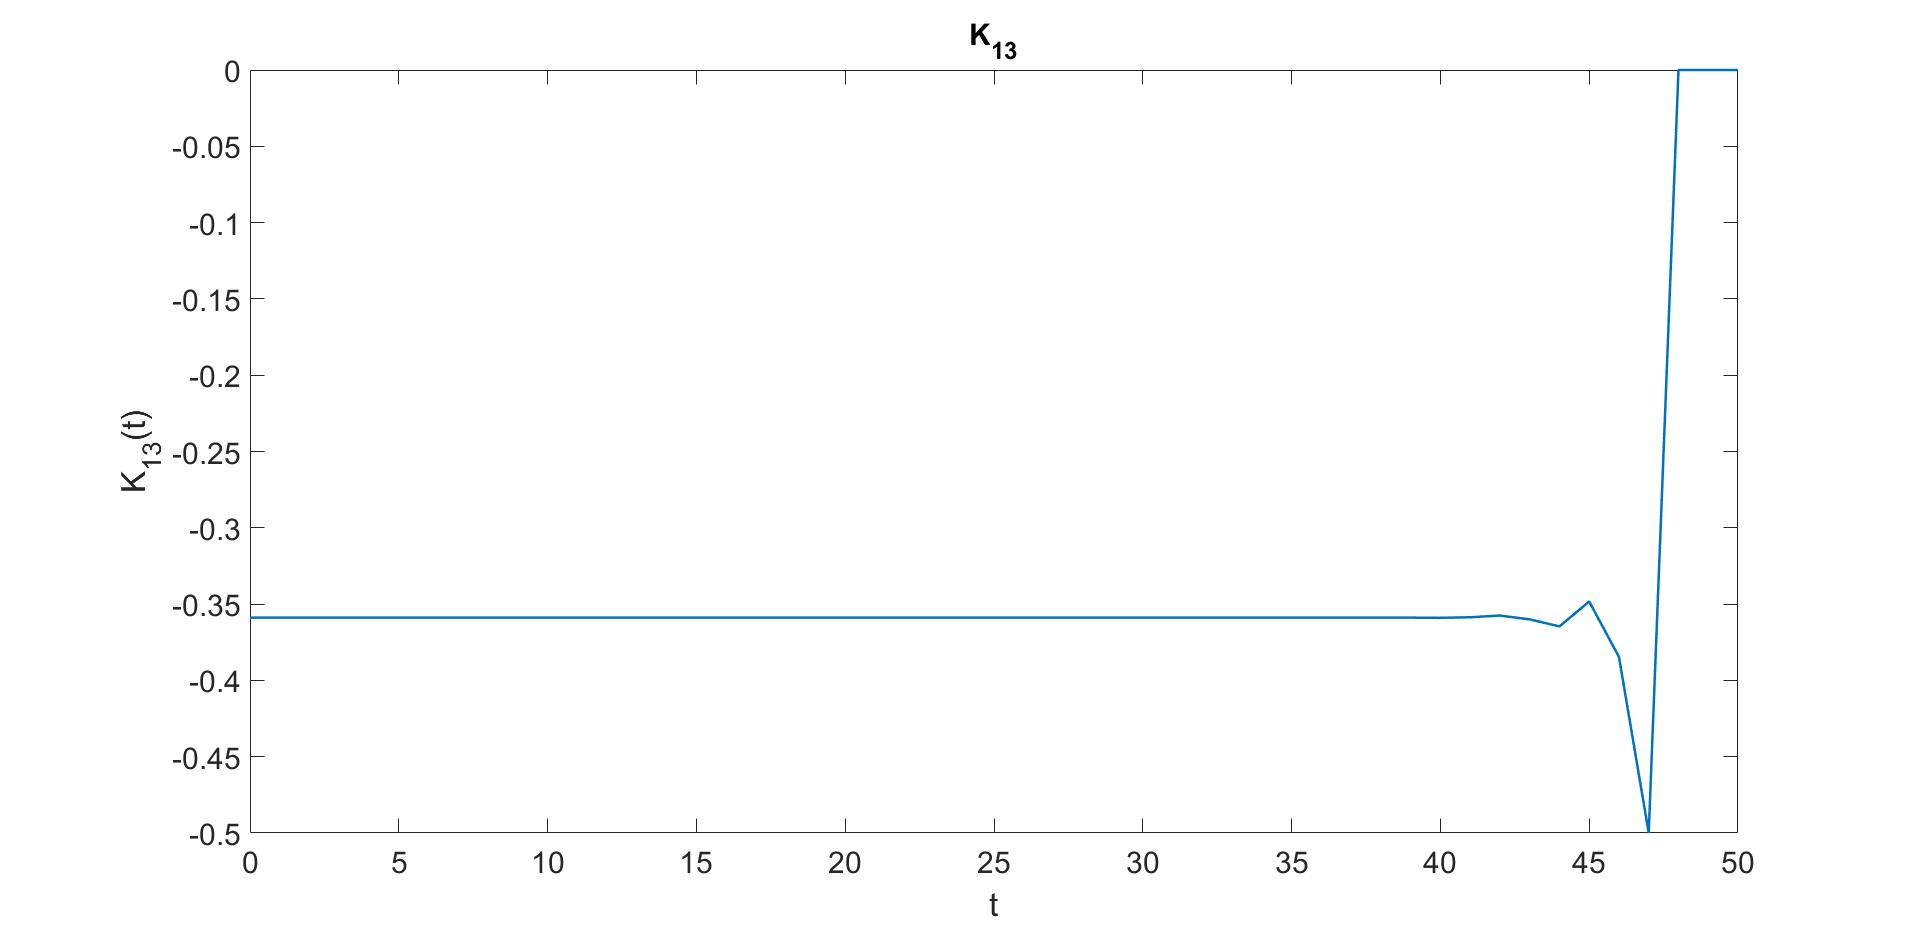
\includegraphics[width=\textwidth,left]{EE 363/HW1/Figures/Figure 3.jpg}
                    \label{fig:Fig_3}
                \end{figure}
        \end{sol}
        \item Find the initial condition $x_{0}$, with norm not exceeding one, that maximizes the optimal value $J$. Plot the optimal $u$ and resulting $x$ for this initial condition.
        \\
        \\
        \begin{sol}
            The optimal cost in state $x_{0}$ is $x_{0}^{T}P_{0}x_{0}$. Since $P$ is symmetric and therefore diagonalizable, we may find maximum and minimum values of its associated quadratic form through maximum eigenvalues and eigenvectors and minimum eigenvalues and eigenvectors, respectively.
            \\
            \\
            Doing so, we find
            \begin{flalign*}
            x_{0}^{opt}
                \begin{bmatrix}
                    6.764 \\
                    7.689 \\
                    2.786
                \end{bmatrix}.
            \end{flalign*}
            
            We may now simulate the system and plot the results.
                \begin{figure}[H]
                    \vspace{-10pt}
                    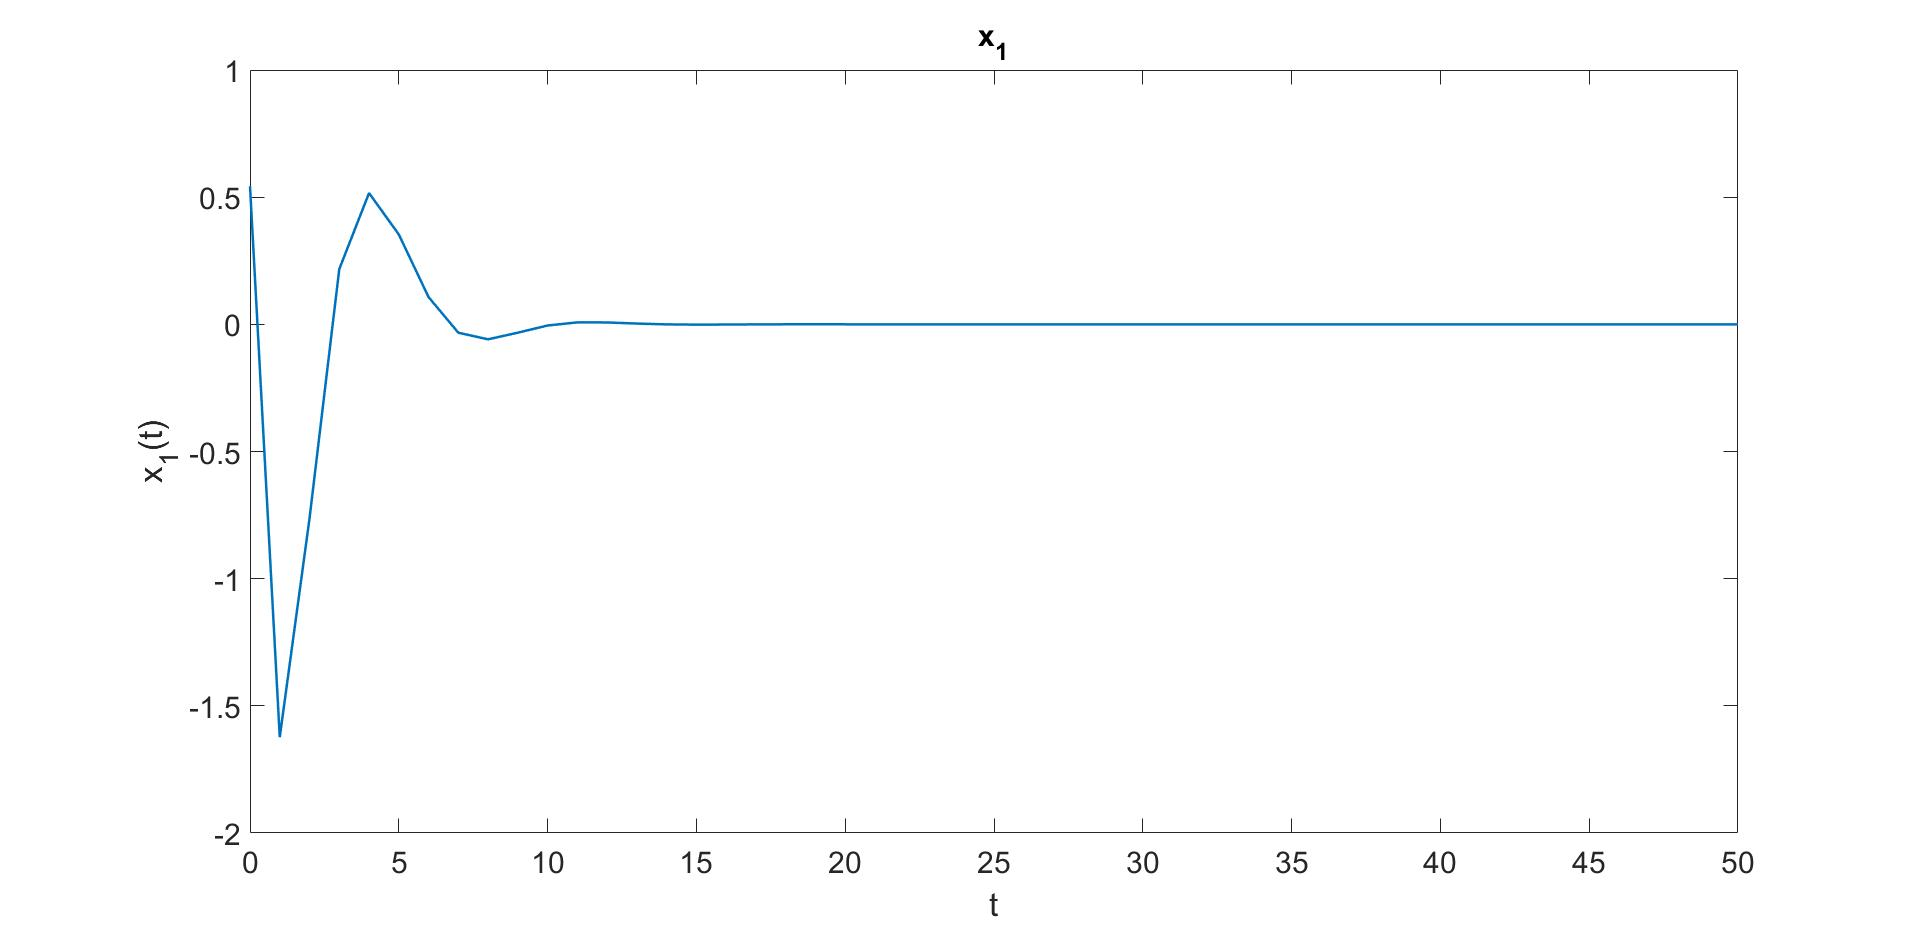
\includegraphics[width=\textwidth,left]{EE 363/HW1/Figures/Figure 4.jpg}
                    \label{fig:Fig_4}
                \end{figure}
                \begin{figure}[H]
                    \vspace{-10pt}
                    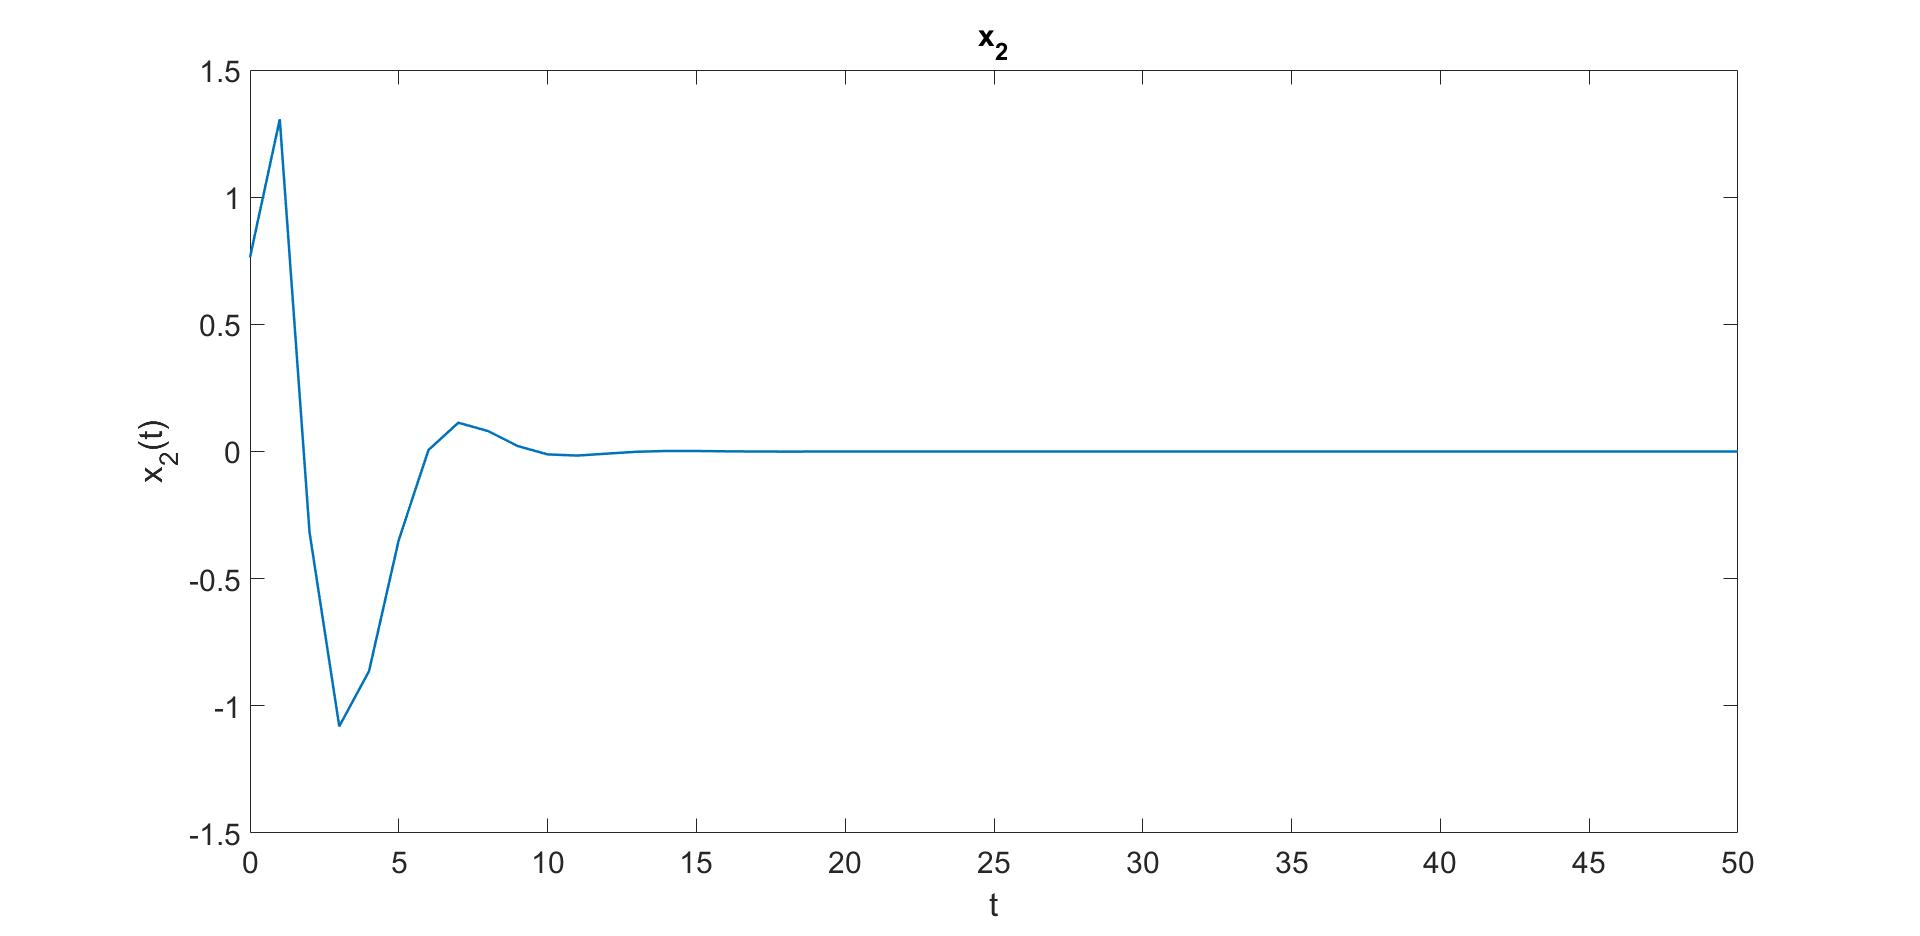
\includegraphics[width=\textwidth,left]{EE 363/HW1/Figures/Figure 5.jpg}
                    \label{fig:Fig_5}
                \end{figure}
                \begin{figure}[H]
                    \vspace{-10pt}
                    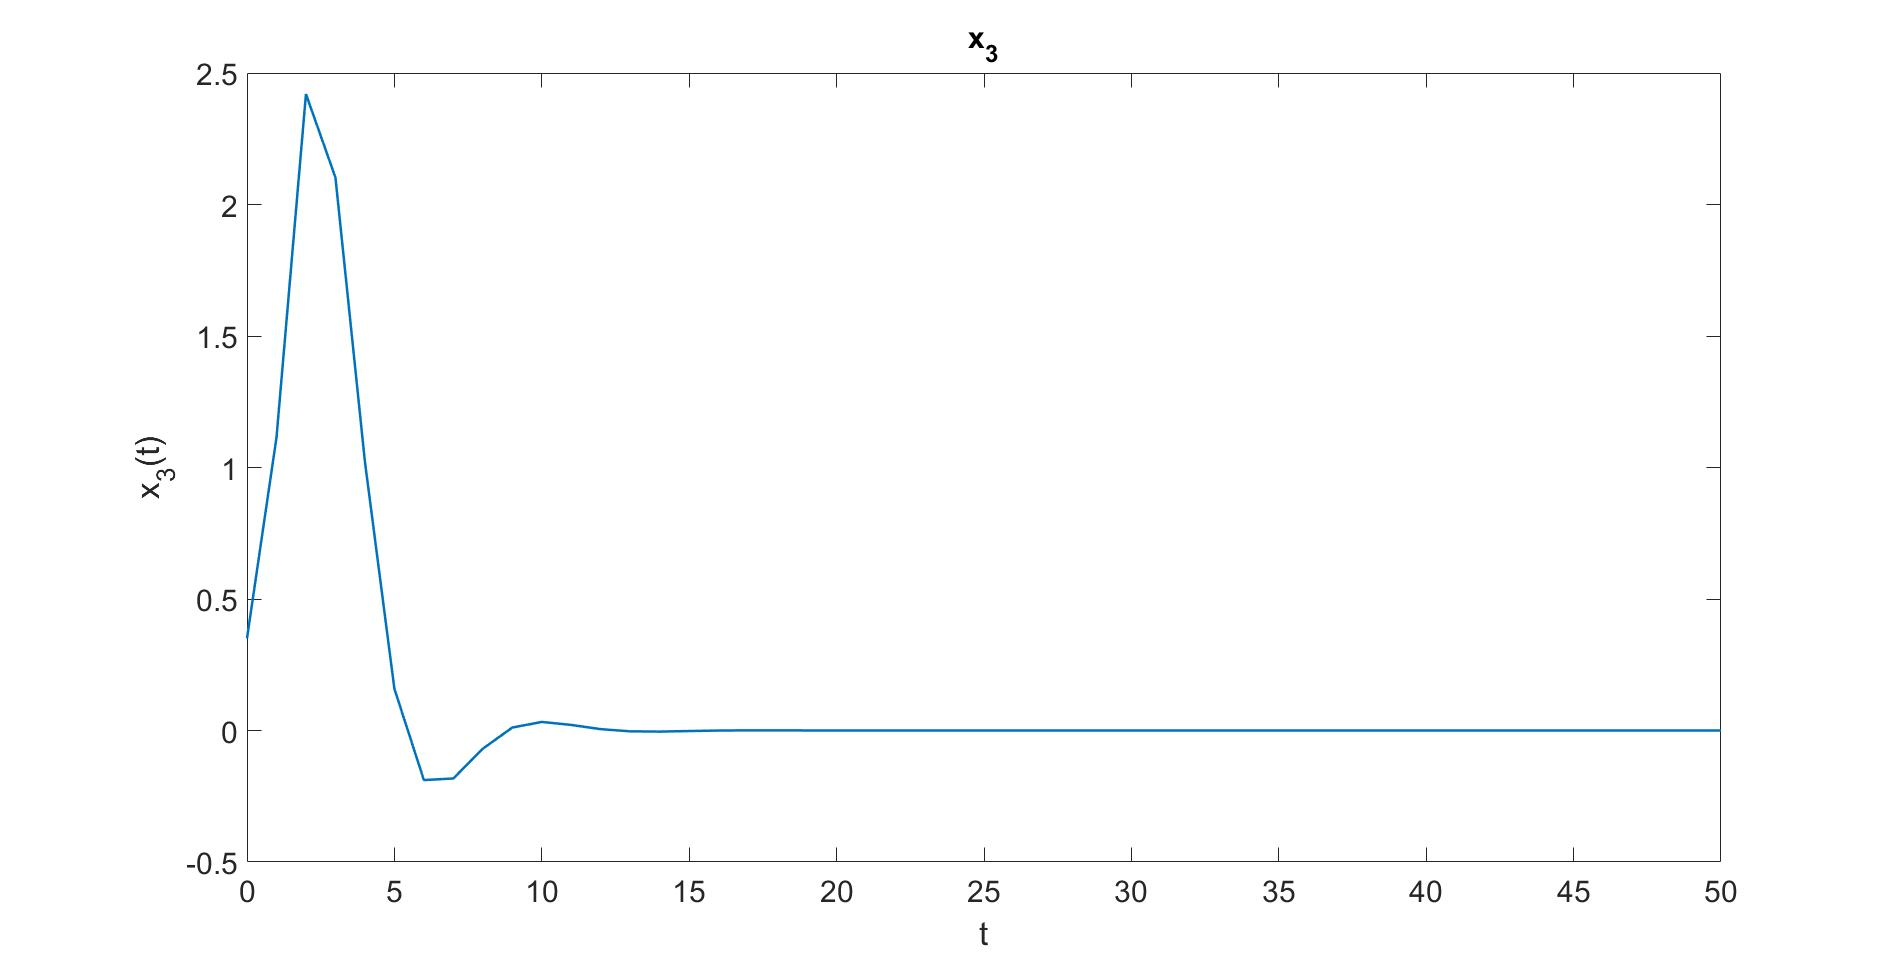
\includegraphics[width=\textwidth,left]{EE 363/HW1/Figures/Figure 6.jpg}
                    \label{fig:Fig_6}
                \end{figure}
                \begin{figure}[H]
                    \vspace{-10pt}
                    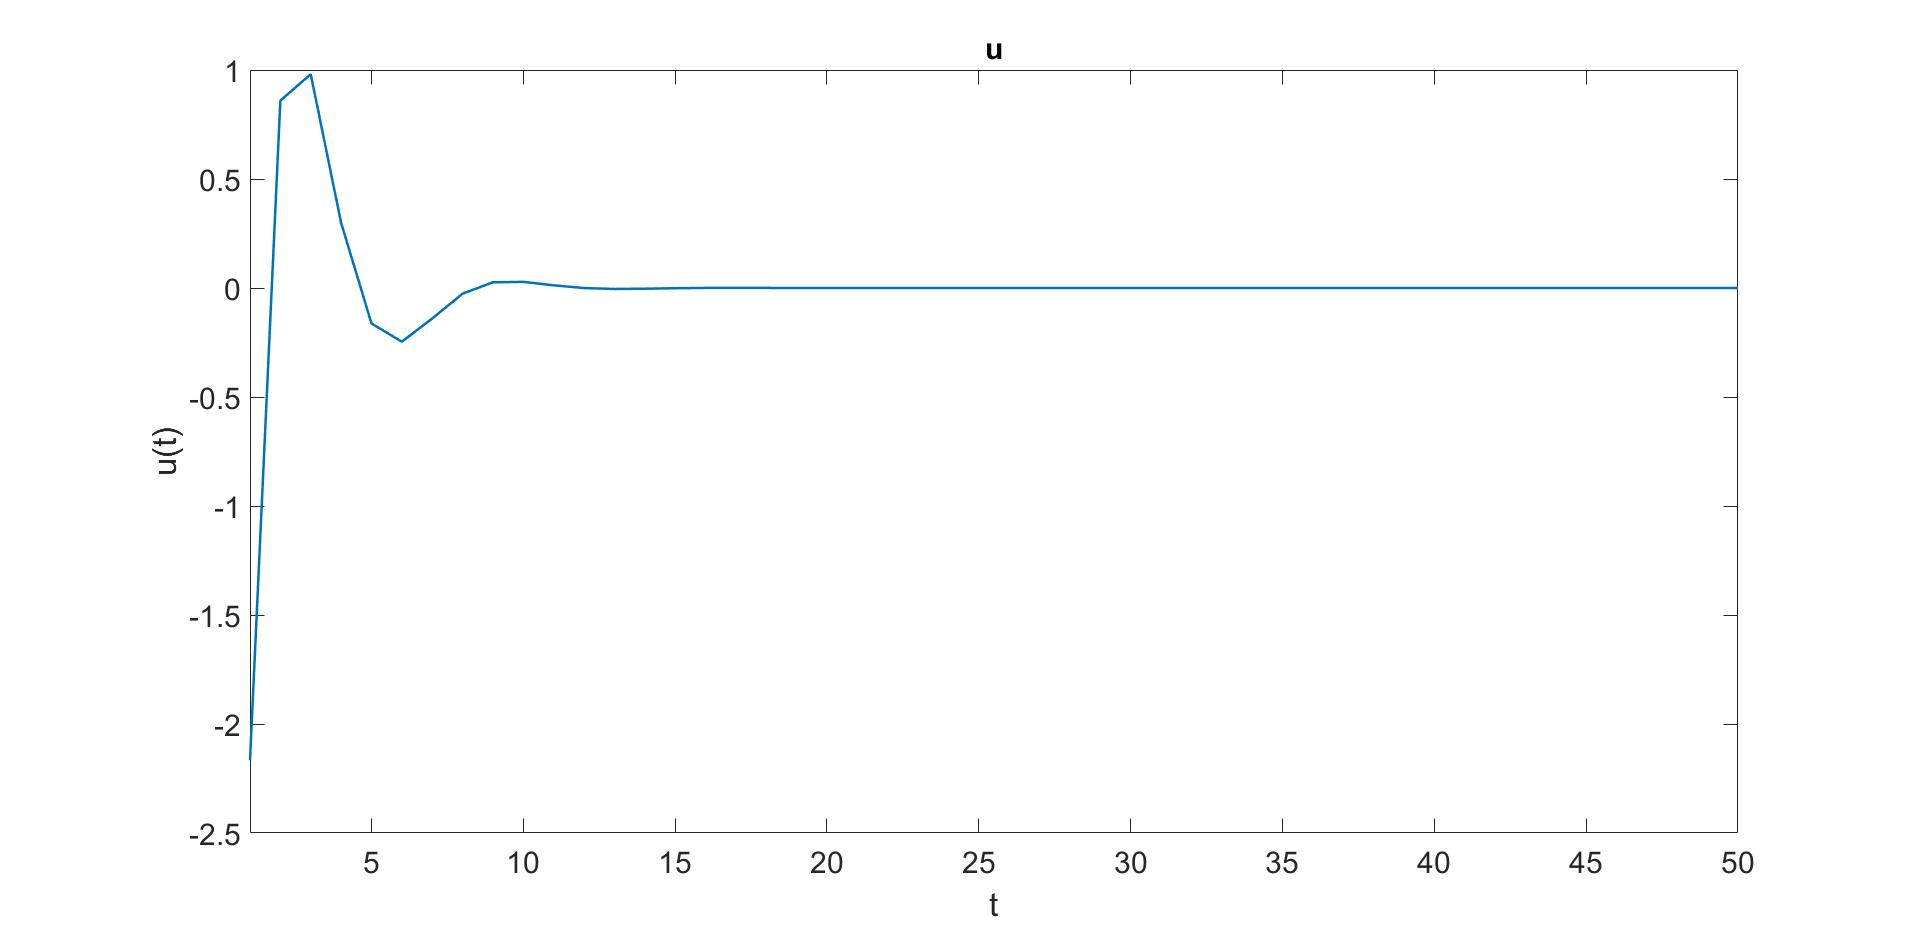
\includegraphics[width=\textwidth,left]{EE 363/HW1/Figures/Figure 7.jpg}
                    \label{fig:Fig_7}
                \end{figure}
        \end{sol}
        \\
        \\
        Please see below MATLAB code:
            
        %%%%
            
\begin{lstlisting}[style=Matlab-editor]
% Given directly from problem
A = [1 0 0; 1 1 0; 0 1 1]; % n-by-n
B = [1; 0; 0;];            % n-by-r
C = [0 0 1];
R = 1;
N = 50;
n = 3;
r = 1;

% Calculate Q
Q = C'*C;

P_t = zeros(n,n,N+1);
K_t = zeros(n,r,N+1);
u_t_lqr = zeros(n,N);
P_t(:,:,N) = Q;
P_eps = zeros(N,1);
K_eps = zeros(N,1);

for i = N:-1:1
    P_t(:,:,i) = Q+A'*P_t(:,:,i+1)*A-A'*P_t(:,:,i+1)*B*((R+B'*...
        P_t(:,:,i+1)*B)^-1)*B'*P_t(:,:,i+1)*A;
    P_eps(i) = 100*max(max(abs((P_t(:,:,i+1)-P_t(:,:,i))./P_t(:,:,i))));
end

for i = 0:N
    K_t(:,:,i+1) = -((R+B'*P_t(:,:,i+1)*B)^-1)*B'*P_t(:,:,i+1)*A;
    if i ~= 0
        K_eps(i) = 100*max(max(abs((K_t(:,:,i+1)-K_t(:,:,i))./...
            K_t(:,:,i))));
    end
end

X = 0:N;

K_11 = reshape(K_t(1,:,:),[N+1 1]);
K_12 = reshape(K_t(2,:,:),[N+1 1]);
K_13 = reshape(K_t(3,:,:),[N+1 1]);

% Solve eigenvalue problem with P_0
[V,D] = eig(P_t(:,:,1));

% Sort eigenvalues
[D_sort,I] = sort(diag(D));

x_0 = -V(:,I(end));
X_s = zeros(n,N+1);
u = zeros(r,N);
X_s(:,1) = x_0;

for i = 1:N
    u(:,i) = K_t(:,:,i)'*X_s(:,i);
    X_s(:,i+1) = A*X_s(:,i)+B*u(:,i);
end

figure(1)

% Plot K_11
plot(X,K_11,'LineWidth',1.5);
xlabel('t','FontSize',18)
ylabel('K_{11}(t)','FontSize',18)
title('K_{11}','FontSize',18)
ax = gca;
% Set x and y font sizes.
ax.XAxis.FontSize = 18;
ax.YAxis.FontSize = 18;
xlim([0 N])

% Make plot size of computer screen
set(gcf, 'Units', 'Normalized', 'OuterPosition', [0 0 1 1]);
% Set background color to white
set(gcf, 'Color', 'w');

figure(2)

% Plot K_12
plot(X,K_12,'LineWidth',1.5);
xlabel('t','FontSize',18)
ylabel('K_{12}(t)','FontSize',18)
title('K_{12}','FontSize',18)
ax = gca;
% Set x and y font sizes.
ax.XAxis.FontSize = 18;
ax.YAxis.FontSize = 18;
xlim([0 N])

% Make plot size of computer screen
set(gcf, 'Units', 'Normalized', 'OuterPosition', [0 0 1 1]);
% Set background color to white
set(gcf, 'Color', 'w');

figure(3)

% Plot K_13
plot(X,K_13,'LineWidth',1.5);
xlabel('t','FontSize',18)
ylabel('K_{13}(t)','FontSize',18)
title('K_{13}','FontSize',18)
ax = gca;
% Set x and y font sizes.
ax.XAxis.FontSize = 18;
ax.YAxis.FontSize = 18;
xlim([0 N])

% Make plot size of computer screen
set(gcf, 'Units', 'Normalized', 'OuterPosition', [0 0 1 1]);
% Set background color to white
set(gcf, 'Color', 'w');

figure(4)

% Plot x_1
plot(X,X_s(1,:),'LineWidth',1.5);
xlabel('t','FontSize',18)
ylabel('x_{1}(t)','FontSize',18)
title('x_{1}','FontSize',18)
ax = gca;
% Set x and y font sizes.
ax.XAxis.FontSize = 18;
ax.YAxis.FontSize = 18;
xlim([0 N])

% Make plot size of computer screen
set(gcf, 'Units', 'Normalized', 'OuterPosition', [0 0 1 1]);
% Set background color to white
set(gcf, 'Color', 'w');

figure(5)

% Plot x_2
plot(X,X_s(2,:),'LineWidth',1.5);
xlabel('t','FontSize',18)
ylabel('x_{2}(t)','FontSize',18)
title('x_{2}','FontSize',18)
ax = gca;
% Set x and y font sizes.
ax.XAxis.FontSize = 18;
ax.YAxis.FontSize = 18;
xlim([0 N])

% Make plot size of computer screen
set(gcf, 'Units', 'Normalized', 'OuterPosition', [0 0 1 1]);
% Set background color to white
set(gcf, 'Color', 'w');

figure(6)

% Plot x_3
plot(X,X_s(3,:),'LineWidth',1.5);
xlabel('t','FontSize',18)
ylabel('x_{3}(t)','FontSize',18)
title('x_{3}','FontSize',18)
ax = gca;
% Set x and y font sizes.
ax.XAxis.FontSize = 18;
ax.YAxis.FontSize = 18;
xlim([0 N])

% Make plot size of computer screen
set(gcf, 'Units', 'Normalized', 'OuterPosition', [0 0 1 1]);
% Set background color to white
set(gcf, 'Color', 'w');

figure(7)

% Plot u
plot(1:N,u,'LineWidth',1.5);
xlabel('t','FontSize',18)
ylabel('u(t)','FontSize',18)
title('u','FontSize',18)
ax = gca;
% Set x and y font sizes.
ax.XAxis.FontSize = 18;
ax.YAxis.FontSize = 18;
xlim([1 N])

% Make plot size of computer screen
set(gcf, 'Units', 'Normalized', 'OuterPosition', [0 0 1 1]);
% Set background color to white
set(gcf, 'Color', 'w');
\end{lstlisting}
            
            %%%%
            
    \end{enumerate}
    \newpage
    \item \textit{Linear Quadratic State Tracking}. We consider the system $x_{t+1}=Ax_{t}+Bu_{t}$. In the conventional LQR problem the goal is to make both the state and the input small. In this problem we study a generalization in which we want the state to follow a desired (possibly nonzero) trajectory as closely as possible. To do this we penalize the \textit{deviations} of the state from the desired trajectory, \textit{i.e.,} $x_{t}-x_{t}^{d}$, using the following cost function:
    \begin{flalign*}
        J &= \displaystyle{\sum_{\tau=0}^{N}(x_{\tau}-x_{\tau}^{d})^{T}Q(x_{\tau}-x_{\tau}^{d})}+\displaystyle{\sum_{\tau=0}^{N}u_{\tau}^{T}Ru_{\tau}},
    \end{flalign*}
    where we assume $Q=Q^{T}\ge0$ and $R=R^{T}\ge0$. (The desired trajectory $x_{\tau}^{d}$ is given). Compared with the standard LQR objective, we have an extra linear term (in $x$) and a constant term.
    
    In this problem you will use dynamic programming to show that the cost-to-go function $V_{t}(z)$ for this problem has the form
    \begin{flalign*}
        z^{T}P_{t}z+2q_{t}^{T}z+r_{t},
    \end{flalign*}
    with $P_{t}=P_{t}^{T}\ge0$. (\textit{i.e.,} it has quadratic, linear, and constant terms).
    
    \begin{enumerate}
        \item Show that $V_{N}(z)$ has the given form.
        \\
        \\
        \begin{sol}
            Since there is no cost-to-go at $t=N$, we have 
            \begin{flalign*}
                V_{N} &= z^{T}P_{N}z = (x_{N}-x_{N}^{d})^{T}Q(x_{N}-x_{N}^{d})=(x_{N}^{T}-(x_{N}^{d})^{T})Q(x_{N}-x_{N}^{d})&& \\
                V_{N} &= (x_{N}^{T}Q-(x_{N}^{d})^{T}Q)(x_{N}-x_{N}^{d})= x_{N}^{T}Qx_{N}-x_{N}^{T}Qx_{N}^{d}-(x_{N}^{d})^{T}Qx_{N}+(x_{N}^{d})^{T}Qx_{N}^{d}&& \\
                V_{N} &= x_{N}^{T}Qx_{N}-(x_{N}^{T}Qx_{N}^{d})^{T}-(x_{N}^{d})^{T}Qx_{N}+(x_{N}^{d})^{T}Qx_{N}^{d}=x_{N}^{T}Qx_{N}-(x_{N}^{d})^{T}Qx_{N}-(x_{N}^{d})^{T}Qx_{N}+(x_{N}^{d})^{T}Qx_{N}^{d}&& \\
                V_{N} &= x_{N}^{T}Qx_{N}-2(x_{N}^{d})^{T}Qx_{N}+(x_{N}^{d})^{T}Qx_{N}^{d}.
            \end{flalign*}
            If we define $r_{N}=(x_{N}^{d})^{T}Qx_{N}^{d}$, $P_{N}=Q$, $x=z$ and $q_{N}=-Q^{T}x_{N}^{d}$, we have
            \begin{flalign*}
                V_{N} &= z^{T}P_{N}z+2q_{N}^{T}z+r_{N},
            \end{flalign*}
            as required.
        \end{sol}
    \end{enumerate}
    \item \textit{A useful determinant identity}. Suppose $X\in\mathbb{R}^{n\times m}$ and $Y\in\mathbb{R}^{m\times n}$.
    \begin{enumerate}
        \item Show that $\text{det}(I+XY)=\text{det}(I+YX)$. \textit{Hint:} Find a block lower triangular matrix $L$ for which 
        \begin{flalign*}
            \begin{bmatrix}
                I & X \\
                -Y & I
            \end{bmatrix}
            &=
            L
            \begin{bmatrix}
                I & X \\
                0 & I
            \end{bmatrix},
        \end{flalign*}
        and use this factorization to evaluate the determinant of this matrix. Then find an upper triangular block matrix $U$ for which 
        \begin{flalign*}
            \begin{bmatrix}
                I & X \\
                -Y & I
            \end{bmatrix}
            &=
            U
            \begin{bmatrix}
                I & 0 \\
                -Y & I
            \end{bmatrix},
        \end{flalign*}
        and repeat.
        \\
        \\
        \begin{sol}
            We first begin with what we are given in the hint:
            \begin{flalign*}
                M=
                \begin{bmatrix}
                    I & X \\
                    -Y & I
                \end{bmatrix}
                &=
                L
                \begin{bmatrix}
                    I & X \\
                    0 & I
                \end{bmatrix}
                =
                \begin{bmatrix}
                    L_{11} & 0 \\
                    L_{21} & L_{22}
                \end{bmatrix}
                \begin{bmatrix}
                    I & X \\
                    0 & I
                \end{bmatrix}
                =
                \begin{bmatrix}
                    L_{11} & L_{11}X       \\
                    L_{21} & L_{21}X+L_{22}
                \end{bmatrix}.
            \end{flalign*}
            Setting each entry in the two matrices equal to each other, we arrive at the following 4 equations:
            \begin{flalign*}
                I &= L_{11}&& \\
                X &= L_{11}X&& \\
                -Y &= L_{21}&& \\
                I &= L_{21}X+L_{22}.
            \end{flalign*}
            From this, we immediately see that $L_{11}=I$ and $L_{21}=-Y$. Substituting, we may find $L_{22}$,
            \begin{flalign*}
                &I = -YX+L_{22}&& \\
                \therefore \ &L_{22} = I+YX.&&
            \end{flalign*}
            Substituting, we use the fact that $\text{det}(T)=\text{det}(T_{11})\text{det}(T_{22})$, where $T$ is a block triangular matrix (this identity can be easily seen by applying Leibniz's formula for the determinant),
            \begin{flalign*}
                \text{det}(M)
                &=
                \text{det}\left(
                \begin{bmatrix}
                    L_{11} & 0 \\
                    L_{21} & L_{22}
                \end{bmatrix}
                \right)
                \text{det}\left(
                \begin{bmatrix}
                    I & X \\
                    0 & I
                \end{bmatrix}
                \right)=\text{det}(L_{11})\text{det}(L_{22})\text{det}(I)\text{det}(I)=\text{det}(L_{11})\text{det}(L_{22})&& \\
                \text{det}(M)&=\text{det}(I)\text{det}(I+YX)&& \\
                \text{det}(M)&=\text{det}(I+YX).
            \end{flalign*}
            We now repeat.
            \begin{flalign*}
                M=
                \begin{bmatrix}
                    I & X \\
                    -Y & I
                \end{bmatrix}
                &=
                U
                \begin{bmatrix}
                    I  & 0 \\
                    -Y & I
                \end{bmatrix}
                =
                \begin{bmatrix}
                    U_{11} & U_{12} \\
                    0      & U_{22}
                \end{bmatrix}
                \begin{bmatrix}
                    I  & 0 \\
                    -Y & I
                \end{bmatrix}
                =
                \begin{bmatrix}
                    U_{11}-U_{12}Y & U_{12} \\
                    -YU_{22}       & U_{22}
                \end{bmatrix}.
            \end{flalign*}
            Setting each entry in the two matrices equal to each other, we arrive at the following 4 equations:
            \begin{flalign*}
                I &= U_{11}-U_{12}Y&& \\
                X &= U_{12}&& \\
                -Y &= -YU_{22}&& \\
                I &= U_{22}.
            \end{flalign*}
            From this, we immediately see that $U_{12}=X$ and $U_{22}=I$. Substituting, we may find $U_{11}$,
            \begin{flalign*}
                &I = U_{11}-XY&& \\
                \therefore \ &U_{11} = I+XY.&&
            \end{flalign*}
            Again, we use the fact that $\text{det}(T)=\text{det}(T_{11})\text{det}(T_{22})$, where $T$ is a block triangular matrix,
            \begin{flalign*}
                \text{det}(M)
                &=
                \text{det}\left(
                \begin{bmatrix}
                    U_{11} & U_{21} \\
                    0      & U_{22}
                \end{bmatrix}
                \right)
                \text{det}\left(
                \begin{bmatrix}
                    I  & 0 \\
                    -Y & I
                \end{bmatrix}
                \right)=\text{det}(U_{11})\text{det}(U_{22})\text{det}(I)\text{det}(I)=\text{det}(U_{11})\text{det}(U_{22})&& \\
                \text{det}(M)&=\text{det}(I)\text{det}(I+XY)&& \\
                \text{det}(M)&=\text{det}(I+XY)=\text{det}(I+YX).
            \end{flalign*}
        \end{sol}
        \item Show that the nonzero eigenvalues of $XY$ and $YX$ are exactly the same.
        \\
        \\
        \begin{sol}
            We first begin with what we are given in the hint as in part (a), but modified slightly:
            \begin{flalign*}
                M=
                \begin{bmatrix}
                    -\lambda I & -\lambda X \\
                    \lambda Y  & -\lambda I
                \end{bmatrix}
                &=
                L
                \begin{bmatrix}
                    I & X \\
                    0 & I
                \end{bmatrix}
                =
                \begin{bmatrix}
                    L_{11} & 0 \\
                    L_{21} & L_{22}
                \end{bmatrix}
                \begin{bmatrix}
                    I & X \\
                    0 & I
                \end{bmatrix}
                =
                \begin{bmatrix}
                    L_{11} & L_{11}X       \\
                    L_{21} & L_{21}X+L_{22}
                \end{bmatrix}.
            \end{flalign*}
            Setting each entry in the two matrices equal to each other, we arrive at the following 4 equations:
            \begin{flalign*}
                -\lambda I &= L_{11}&& \\
                -\lambda X &= L_{11}X&& \\
                \lambda Y &= L_{21}&& \\
                -\lambda I &= L_{21}X+L_{22}.
            \end{flalign*}
            From this, we immediately see that $L_{11}=-\lambda I$ and $L_{21}=\lambda Y$. Substituting, we may find $L_{22}$,
            \begin{flalign*}
                &-\lambda I = \lambda YX+L_{22}&& \\
                \therefore \ &L_{22} = I+YX.&&
            \end{flalign*}
            Substituting, we use the fact that $\text{det}(T)=\text{det}(T_{11})\text{det}(T_{22})$, where $T$ is a block triangular matrix (this identity can be easily seen by applying Leibniz's formula for the determinant),
            \begin{flalign*}
                \text{det}(M)
                &=
                \text{det}\left(
                \begin{bmatrix}
                    L_{11} & 0 \\
                    L_{21} & L_{22}
                \end{bmatrix}
                \right)
                \text{det}\left(
                \begin{bmatrix}
                    I & X \\
                    0 & I
                \end{bmatrix}
                \right)=\text{det}(L_{11})\text{det}(L_{22})\text{det}(I)\text{det}(I)=\text{det}(L_{11})\text{det}(L_{22})&& \\
                \text{det}(M)&=\text{det}(I)\text{det}(I+YX)&& \\
                \text{det}(M)&=\text{det}(I+YX).
            \end{flalign*}
            We now repeat.
            \begin{flalign*}
                M=
                \begin{bmatrix}
                    I & X \\
                    -Y & I
                \end{bmatrix}
                &=
                U
                \begin{bmatrix}
                    I  & 0 \\
                    -Y & I
                \end{bmatrix}
                =
                \begin{bmatrix}
                    U_{11} & U_{12} \\
                    0      & U_{22}
                \end{bmatrix}
                \begin{bmatrix}
                    I  & 0 \\
                    -Y & I
                \end{bmatrix}
                =
                \begin{bmatrix}
                    U_{11}-U_{12}Y & U_{12} \\
                    -YU_{22}       & U_{22}
                \end{bmatrix}.
            \end{flalign*}
            Setting each entry in the two matrices equal to each other, we arrive at the following 4 equations:
            \begin{flalign*}
                I &= U_{11}-U_{12}Y&& \\
                X &= U_{12}&& \\
                -Y &= -YU_{22}&& \\
                I &= U_{22}.
            \end{flalign*}
            From this, we immediately see that $U_{12}=X$ and $U_{22}=I$. Substituting, we may find $U_{11}$,
            \begin{flalign*}
                &I = U_{11}-XY&& \\
                \therefore \ &U_{11} = I+XY.&&
            \end{flalign*}
            Again, we use the fact that $\text{det}(T)=\text{det}(T_{11})\text{det}(T_{22})$, where $T$ is a block triangular matrix,
            \begin{flalign*}
                \text{det}(M)
                &=
                \text{det}\left(
                \begin{bmatrix}
                    U_{11} & U_{21} \\
                    0      & U_{22}
                \end{bmatrix}
                \right)
                \text{det}\left(
                \begin{bmatrix}
                    I  & 0 \\
                    -Y & I
                \end{bmatrix}
                \right)=\text{det}(U_{11})\text{det}(U_{22})\text{det}(I)\text{det}(I)=\text{det}(U_{11})\text{det}(U_{22})&& \\
                \text{det}(M)&=\text{det}(I)\text{det}(I+XY)&& \\
                \text{det}(M)&=\text{det}(I+XY)=\text{det}(I+YX).
            \end{flalign*}
        \end{sol}
    \end{enumerate}
\end{enumerate}

\end{document}
